\subsection{Ecuación de recurrencia de primer orden}

\begin{frame}
\frametitle{\subsecname}

\begin{definition}
	Una \textbf{ecuación de recurrencia lineal de primer orden} relaciona entradas consecutivas en una sucesión mediante una ecuación de la forma
	\begin{equation}\label{eq:firstoder}
		S_{n+1}=aS_{n}+c,\quad\forall n\in\mathds{N},
	\end{equation}
	donde $a\neq0$ y la condicional inicial es $S_{0}$.
\end{definition}

\begin{claim}
	La solución general de~\eqref{eq:firstoder} se divide en dos casos:
	\begin{description}
		\item[Primer caso] Si $a=1$, entonces  \[ S_{n}= S_{0}+nc,\quad\forall n\in\mathds{N} \].
		\item[Segundo caso] Si $a\neq1$, entonces \[ S_{n}=a^{n}\left[S_{0}-\frac{c}{1-a}\right]+\frac{c}{1-a},\quad\forall n\in\mathds{N}. \]
	\end{description}
\end{claim}
\end{frame}

\subsubsection{Torre de Hanói}

\begin{frame}
\frametitle{\subsubsecname}

\begin{minipage}{0.45\paperwidth}
Considere la ecuación de recurrencia~\eqref{eq:firstoder} \[ S_{n}=2S_{n-1}+1,\quad\forall n\geq2, \] donde:
\begin{itemize}
	\item $n$ denota el número de discos y
	\item $S_{n}$ es el mínimo número de movimientos necesario para transportar los $n$ discos desde una aguja a otra.
\end{itemize}
\end{minipage}
\hfill
\begin{minipage}{0.45\paperwidth}
	\begin{figure}[H]
		\centering
		
\includegraphics[width=0.4\paperwidth]{hanoi}
		\caption{El objetivo es trasladar los discos de una aguja a otra bajo ciertas condiciones.}
	\end{figure}
\end{minipage}
\end{frame}

\subsection{Ecuación de recurrencia lineal de segundo orden}

\begin{frame}
\frametitle{\subsecname}

\begin{definition}
	Una \textbf{ecuación de recurrencia lineal de segundo orden} relaciona entradas consecutivas en una secuencia mediante una ecuación de la forma
	\begin{equation}\label{eq:secondorder}
	S_{n+2}=aS_{n+1}+bS_{n}+c,\quad\forall n\in\mathds{N},
	\end{equation}
	donde $ab\neq0$. Cuando $c=0$, la ecuación de recurrencia se dice que es \textbf{homogénea}.
\end{definition}

\begin{definition}
	La \textbf{ecuación característica} de~\eqref{eq:secondorder} homogénea es $x^{2}-ax-b=0$ que tiene raíces \[ r_{1}=\frac{a+\Delta}{2}\quad\text{y}\quad r_{2}=\frac{a-\Delta}{2}\quad\text{donde }\Delta=\sqrt{a^{2}+4b}. \]
\end{definition}

\begin{theorem}
	La solución general de~\eqref{eq:secondorder} homogénea es
	\begin{align*}
	S_{n}&=A{\left(r_{1}\right)}^{n}+B{\left(r_{2}\right)}^{n}&\text{si }r_{1}\neq r_{2}\phantom{r_{2}r_{2}}\quad\left(\Delta\neq0\right),\\
	S_{n}&=A{\left(r\right)}^{n}+Bn{\left(r\right)}^{n}&\text{si }r_{1}=r_{2}=r\quad\left(\Delta=0\right).
	\end{align*}
\end{theorem}

%\begin{proof}
%	Por favor,~\citeauthor[ver][357]{Jenkyns2018}.
%\end{proof}

\end{frame}

\subsubsection{Un modelo de la cunicultura}

\begin{frame}
\frametitle{\subsubsecname}

Considere la ecuación de recurrencia \[ F_{n}=F_{n-1}+F_{n-2},\quad\forall n\geq2, \] llamada \textbf{ecuación de Fibonacci}.

\

\begin{minipage}{0.45\paperwidth}
Fibonacci partía de ciertas hipótesis, a saber:
	\begin{itemize}
		\item Los conejos viven eternamente.
		\item Cada mes, un par de adultos de distinto sexo da lugar a un nuevo par de conejos de distinto sexo.
		\item Cada conejo se hace adulto a los dos meses de vida, momento en el que comienza a tener descendencia.
	\end{itemize}
\end{minipage}
\hfill
\begin{minipage}{0.45\paperwidth}
	\begin{figure}[H]
		\centering
		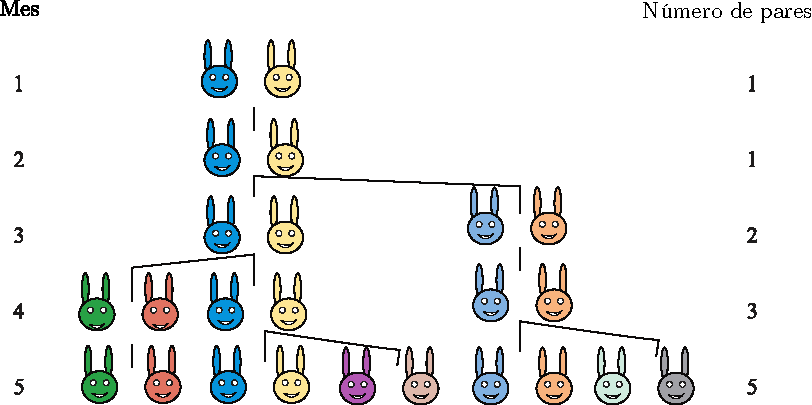
\includegraphics[width=0.4\paperwidth]{rabbits}
		\caption{La cantidad de conejos en función de los meses transcurridos.}
	\end{figure}
\end{minipage}

\end{frame}